\chapter{Introducción}
\label{Introducción}

%Historia de como se presenta la oportunidad de hacer este trabajo final
Ante la propuesta del profesor Petrashin de desarrollar un trabajo final en base al tema presentado en microelectrónica II, Control Potencia con circuitos integrados (\textit{Power Management Integrated Circuits, PMIC}), se desarrolla el presente trabajo final. Partiendo de tesis de doctorado (referencia) se realiza una investigación del estado del arte y se estudia los conversores DC-DC. Por lo que se delimita el alcance del Trabajo Final con los requerimientos funcionales y no funcionales.
\section{Requerimientos Funcionales y No funcionales}
Para poder realizar el trabajo dentro de un tiempo comprensible, y no tenga un alcance ¿uperior/desviado al titulo de ingeniero electrónico, se pauta la tabla \ref{requerimientos-tabla}.
\begin{table}[h]
\resizebox{\textwidth}{!}{\begin{tabular}{|c|c|c|}
    \hline
    Requerimientos Funcionales & Requerimientos No Funcionales\\
    \hline
    Potencia máxima de panel solar de 300W & Emplear un conjunto de paneles solares de la universidad UCC\\
    \hline
    Corroborar distintos métodos de MPPT & Disponibilidad local de componentes\\
    \hline
    Guardar los datos reales & Fácil instalación y replica\\
    \hline
\end{tabular}}
\caption{Requerimientos funcionales y no funcionales}
\label{requerimientos-tabla}
\end{table}

\section{Zona de trabajo}
Se desarrolla el trabajo teniendo en cuenta que se implementa/implementara en el sector de energías renovables en el exterior de la facultad de ingenierías de la Universidad Católica de Córdoba. Un sector aislado del edificio ubicado en las coordenadas -31.486791, -64.240144. Los paneles presentes son de código KS75T de la empresa SOLARTEC®, Figura \ref{fig:panelsolarencampo}, cuya curva característica de potencia se observa en la Figura \ref{fig:curvadepaneldata}
\begin{figure}
    \centering
    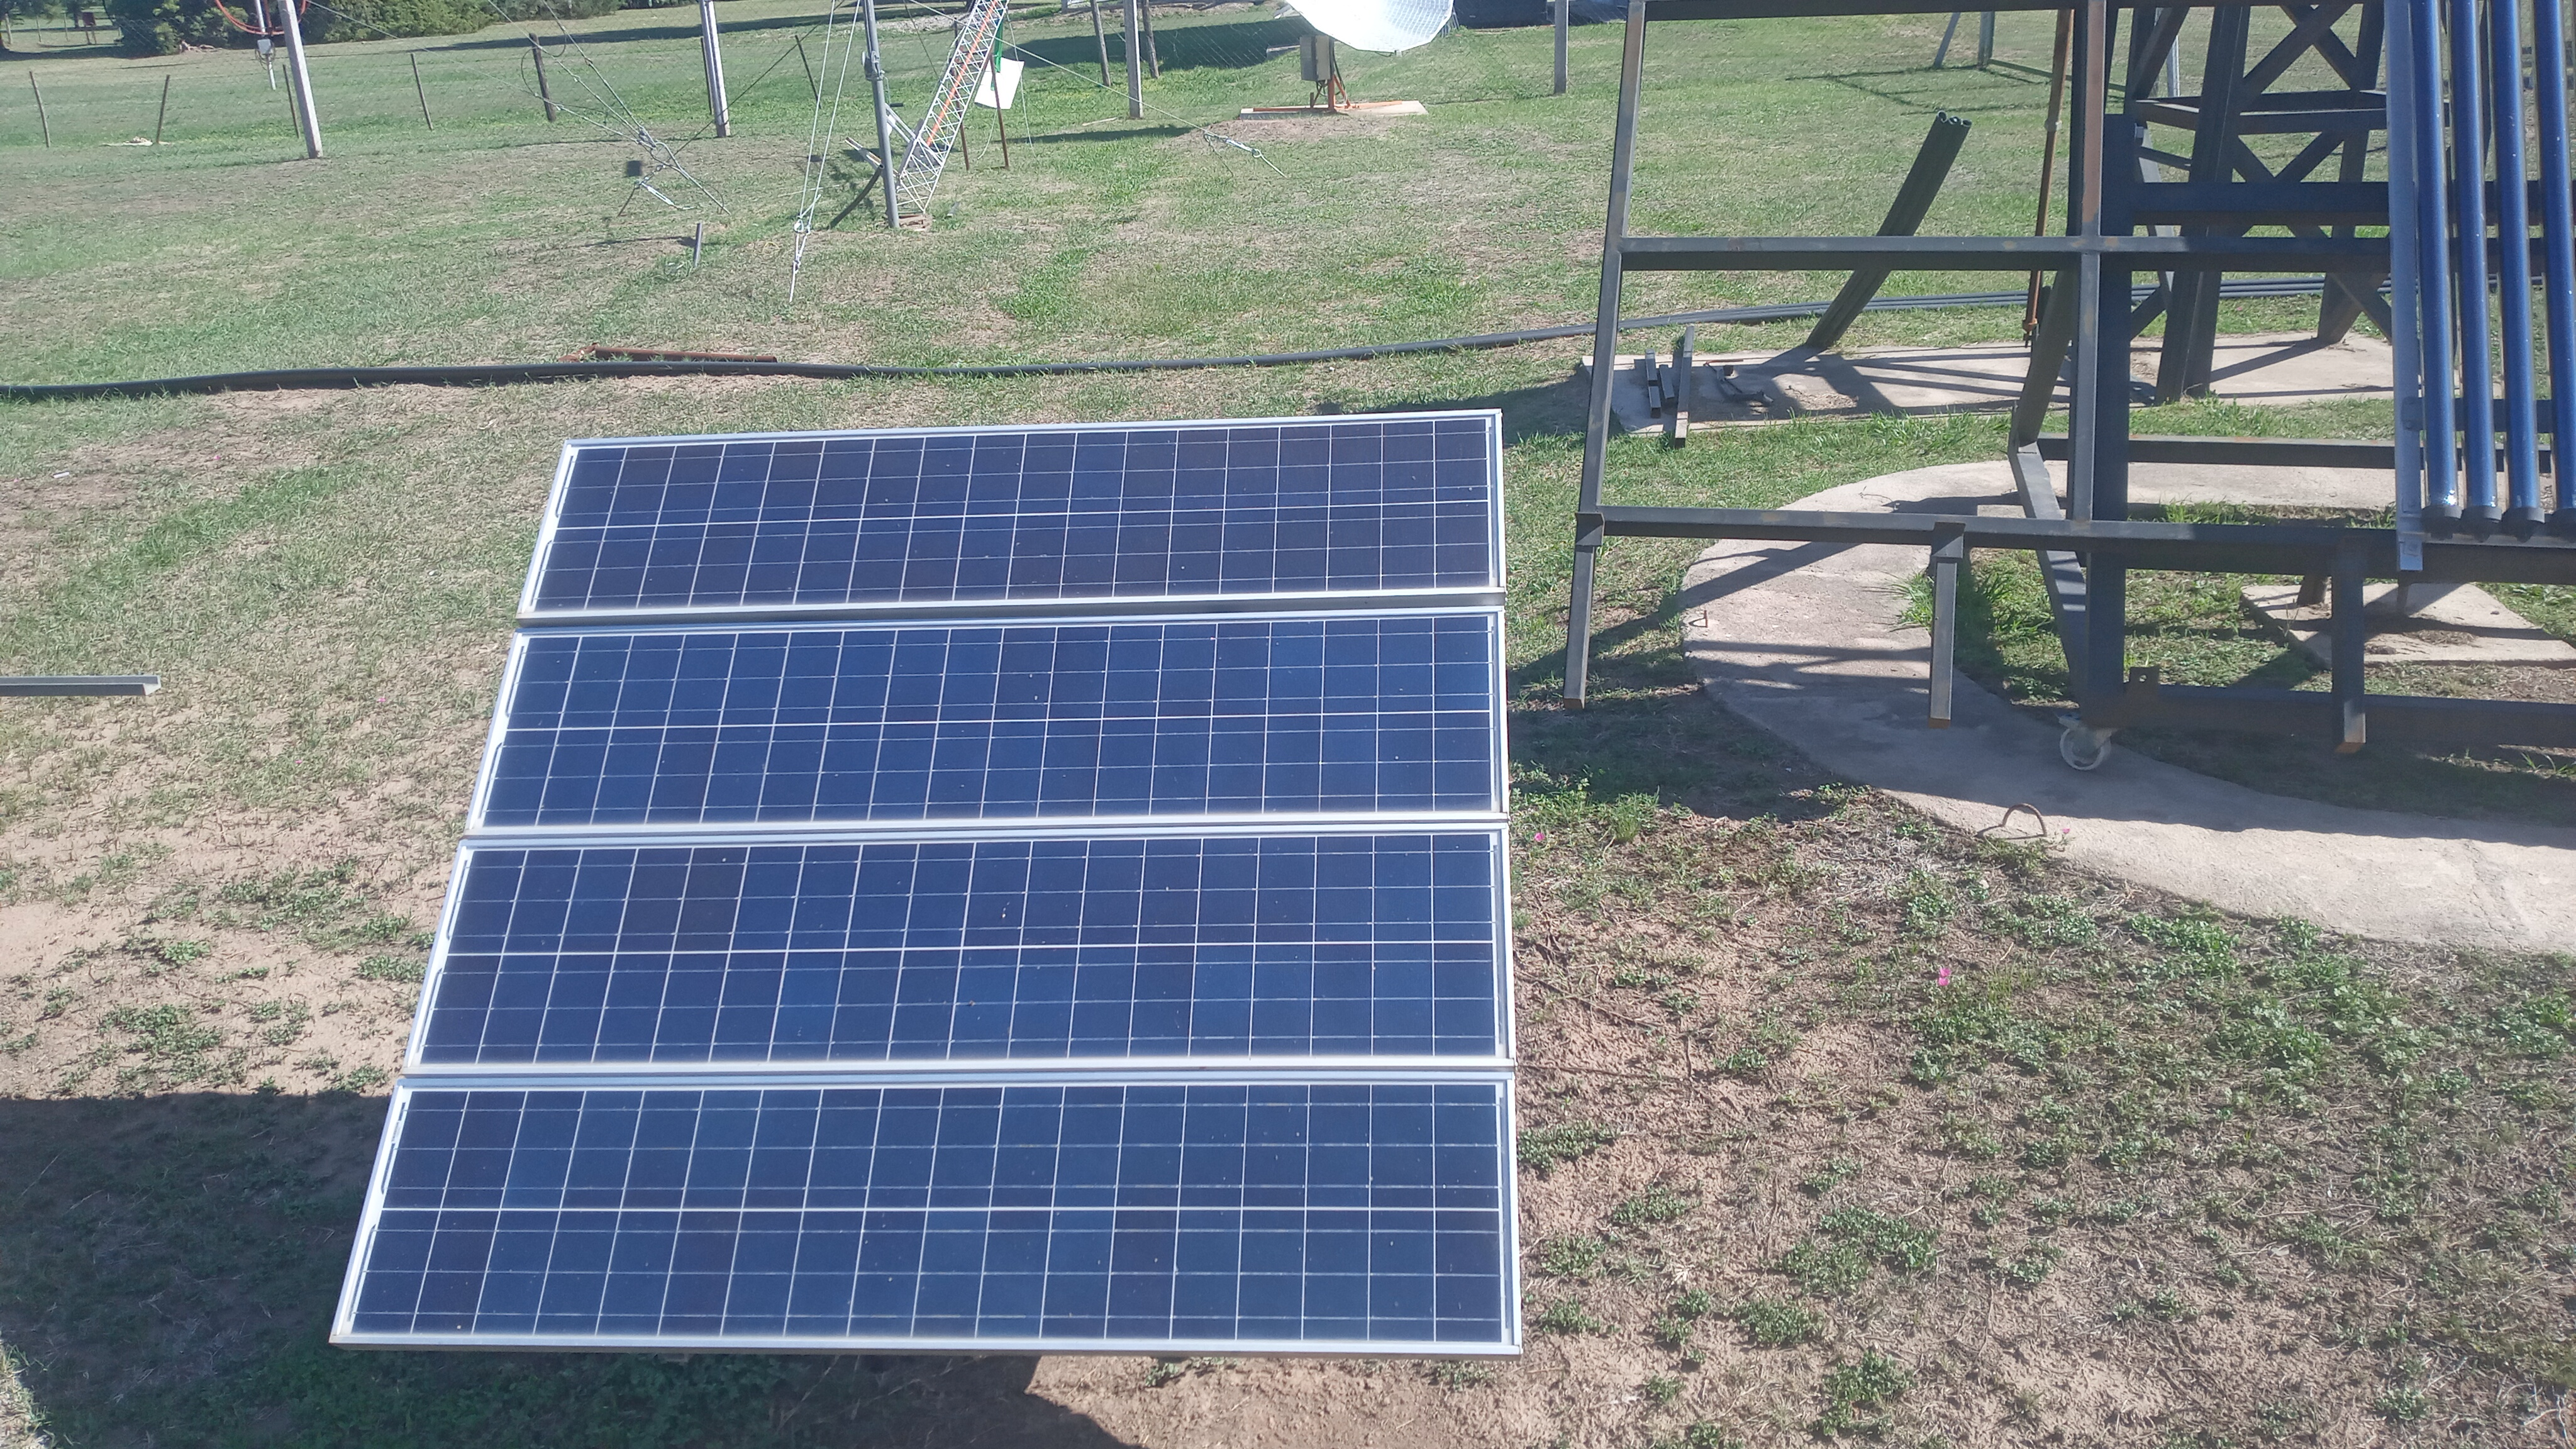
\includegraphics[width=1\linewidth,frame]{imagenes/panelsolarencampofrontal.jpg}
    \caption{Paneles solares en campo}
    \label{fig:panelsolarencampo}
\end{figure}
\begin{figure}
    \centering
    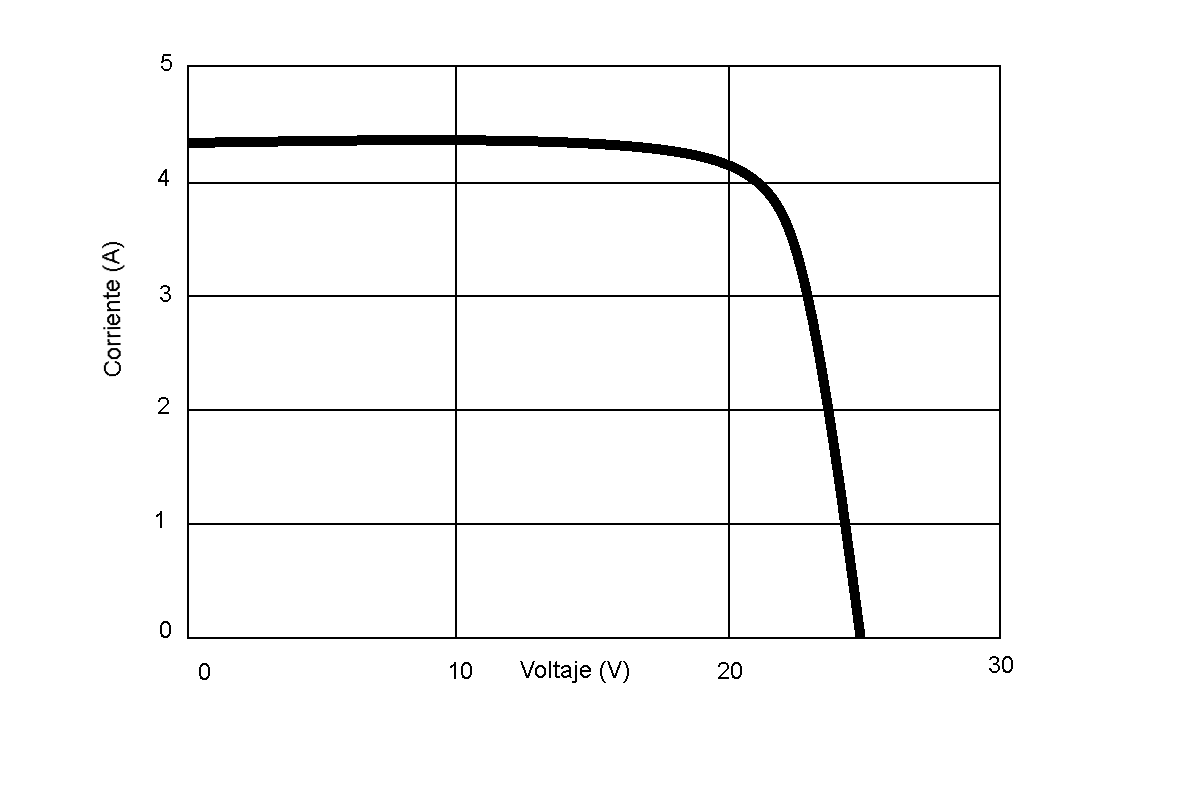
\includegraphics[width=1\linewidth,frame]{imagenes/curvapaneldata.png}
    \caption{Curva característica de Panel Solar}
    \label{fig:curvadepaneldata}
\end{figure}
